\section{Implementation and Results}

After completing the service mesh setup it is time to examine the necessary steps to apply the showcases stated in \autoref{sec:showcases-1} with \linkerd{}, how the results look like and some pitfalls we have overcome.

Since functionality and APIs vary in time, the following table shows the versions of technologies we use:
\begin{table}[h]
\centering	
\begin{tabular}{c|c}
	Technology & Version \\\hline
	\textsc{Docker} & 20.10.3\\\hline
	\textsc{Minikube} & 1.17.1\\\hline
	\kubernetes & 1.20.2\\\hline
	\linkerd & 2.9.3 \\
\end{tabular}
\vspace{0.25mm}
\caption{Technologies and Versions in our Project}
\label{tab:versions}
\end{table}

Services are built into \textsc{Docker}-images.
To use only one machine for development we used \textsc{Minikube}.
Within this \kubernetes{} and \linkerd{} run.

\subsection{Showcases Implementation}
With the exception of "Acess Policies" we implemented and controlled with \linkerd{} the challenges stated in \autoref{sec:showcases-1}.

\subsubsection{Encryption}
From the second that a service is injected by \linkerd{} and applied to the cluster, all communication to that service is automatically encrypted.
This holds not only for our self-implemented communication but also for metrics- and tap-services.
Since the communication is proxied by \linkerd{} it activates certificate distribution and encryption out-of-box.

If you don't want to use this feature, you can disable by overwriting the \linkerd{} configuration.
The following command will generate an updated YAML-configuration you can apply in \kubernetes{}.
\begin{lstlisting}
linkerd upgrade \
  --disable-identity \
  --disable-tap
\end{lstlisting}
Note: Once this configuration is applied, there will be no encryption neither in communication between services nor in tap- and metrics-services.

\subsubsection{Canary Deployment}
\label{sec:canary-result}
In first place we have to deploy a new version of the \textsc{name-service} next to the existing one.
The deployment is done the same way but with a different name (\lstinline|nameapi-v2|).
New Version of \textsc{name-service} is similar to the old one but returns a different string (forename \textit{and} surname) while API stays the same.
There are no changes in \textsc{hello-world-service} necessary.

Until now the new version is not used.
We have to define a traffic split showed in \autoref{lst:traffic-split}.

\begin{lstlisting}[caption={YAML configuration of 90/10 traffic split. 90\% of requests are routed to \lstinline|nameapi| and 10\% to \lstinline|nameapi-v2|.}, label={lst:traffic-split}]
apiVersion: split.smi-spec.io/v1alpha1
kind: TrafficSplit
metadata:
	name: nameapi-split
spec:
	service: nameapi
	backends:
	- service: nameapi
		weight: 90
	- service: nameapi-v2
		weight: 10
\end{lstlisting}

In the \lstinline|spec|-section we define two backends for the service \lstinline|nameapi|.
The argument \lstinline|weight| defines a split ratio.
90\% of traffic should be routed to the existing service with the name \lstinline|nameapi|, 10\% to the new one \lstinline|nameapi-v2|.

Right after applying this configuration, \linkerd{} dashboard shows a new section for traffic splits.
In \autoref{fig:results-traffic-split-weights} \linkerd{} visualizes the routed requests.
We can see the defined weights and the current requests per second (RPS), that are split according.

\begin{figure}
	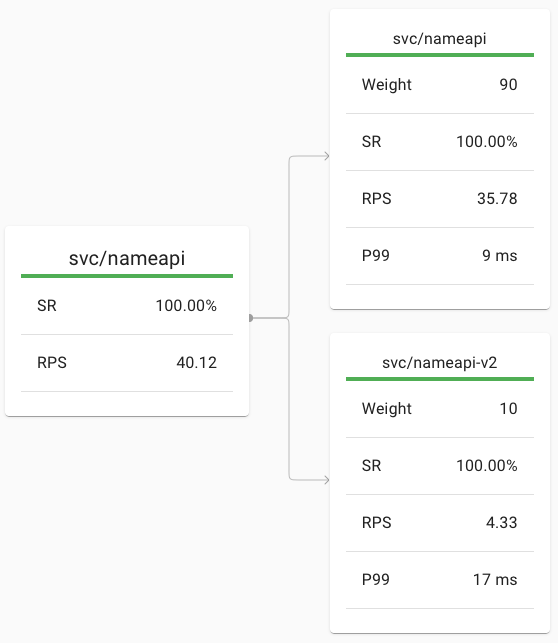
\includegraphics[width=\columnwidth]{img/results-traffic-split-weights}
	\caption{\linkerd{} dashboard displays the weights of the 90/10 traffic split.}
	\label{fig:results-traffic-split-weights}
\end{figure}

The \textsc{hello-world-service} stays unchanged, but requests the new version of \textsc{name-service} every tenth request without knowing.
The deployment section of \textsc{hello-world-service} in \linkerd{} dashboard now renders a delegation tree pictured in \autoref{fig:results-traffic-split-tree} showing that \textsc{hello-world-service} requests both versions of \textsc{name-service}.

\begin{figure}
	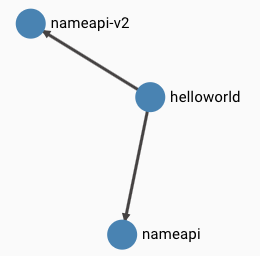
\includegraphics[width=.4\columnwidth]{img/results-traffic-split-tree}
	\centering
	\caption{Delegation tree of \textsc{hello-world-service} after traffic split.}
	\label{fig:results-traffic-split-tree}
\end{figure}




\subsubsection{Access Policies}
To restrict the access to the \textsc{name-service} is the only challenge we did not made.
Access policies is a topic often called in context of service meshes.
But until now there is no support on the part of \linkerd{}.
On GitHub you'll find an open issue from 2019 asking for support of \kubernetes{}' \textit{Network Policies}\footnote{
	See \url{https://github.com/linkerd/linkerd2/issues/2746}	
}.
But for the last two years it is still open.
	
We tried to implement it with Network Policies but have not made it due to time constraints.
It is not just trivial because you have to restrict \linkerd{}'s sidecars rather than services itself.
Sure it will be possible with \kubernetes{} to manage it, but it's not a feature of \linkerd{}.
This is why we dropped this showcase in order to finish the other four.

\subsubsection{Load Balancing}
\label{sec:load-result}
To show the integrated load balancing of \linkerd{} we defined three replicas of the \textsc{goodbye-world-service}.
Therefore we set In the deployment configuration at the \lstinline|spec|-section the count of replicas up to three	 (\lstinline|replicas: 3|).
Now \kubernetes{} will provide three pods running the \textsc{goodbye-world-service}.
Since we injected the configuration file by \linkerd{} all replicas are within the service mesh and load balancing takes place out-of-box.

\autoref{fig:results-load-balance} shows the pods list of \linkerd{} dashboard in the deployment view of \textsc{goodbye-world-service}.
We can see that requests are balanced equally to each pod.

\begin{figure}
	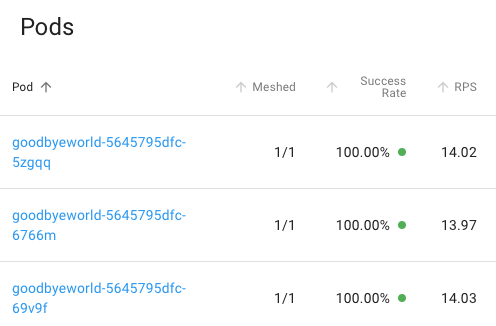
\includegraphics[width=\columnwidth]{img/results-load-balance}
	\caption{The \textsc{goodbye-world-service} deployment shows all three replicas balancing the request-load.}
	\label{fig:results-load-balance}
\end{figure}

\subsubsection{Central Monitoring and Logging}
\label{sec:log-result}
As we can see \linkerd{} comes with a dashboard showing the current state of the service mesh (see images in \autoref{sec:canary-result} and \autoref{sec:load-result}).
To collect the so called "golden metrics" \linkerd{} brings \textsc{Prometheus} which is out-of-box connected to each pod.
With this we can see \textit{who} is talking \textit{how much} to \textit{whom}.
Next to the \linkerd{} dashboard there is a \textsc{Grafana} component for each deployment \linkerd{} provides automatically.
Different from the dashboard of \linkerd{} \textsc{Grafana} shows temporal progression of the metrics.

To receive the logs of a service you may use the \kubernetes{} command \lstinline|kubectl logs <pod> <service>|
	\footnote{
		There was an own implementation for logs in \linkerd{} (\lstinline|linkerd logs|). 
		It was removed somewhere about version 2.4 since it overlapped with \lstinline|kubectl logs|.
		Read more in this GitHub discussion:\\
		\url{https://github.com/linkerd/linkerd2/discussions/5790}
	}.

\subsection{Pitfalls}
This section is for everybody wanting to reproduce showcases above.
Here we stated most important hints for which we would have been grateful if we had had them at the beginning:
\begin{itemize}
	\item First tip: Bring some time.\\
	To use \linkerd{} you have to acquire knowledge about \kubernetes{} and the Unix-Shell.
	There is no way to use \linkerd{} without \kubernetes{}.
	In many commands you rather have to call \lstinline|kubectl| than \lstinline|linkerd|.
	
	Since this project was time-boxed, we weren't able to finish the "Access Policies" because of this huge period of vocational adjustment.
	
	\item Give enough RAM.\\
	In the documentation of \textsc{Minikube} we found, that 2 GB of RAM should be enough\footnote{
		See \url{https://minikube.sigs.k8s.io/docs/start/}
	}.
	But for running \linkerd{} inside it wasn't. 
	After a few hours of running the operating system began to swap memory and \kubernetes{} was unusable. 
	Provisioning up to 4 GB solved this problem.

	\item Connect to \textsc{Minikube} Environment.\\
	Building your Dockerfile into an image does not provide it for \textsc{Minikube}.
	To make it available for \textsc{Minikube} you have to run the following command in \textit{every} shell-session you want to build:
	\lstinline|eval $(minikube -p minikube docker-env)|
	This will connect your local \textsc{Docker}-CLI to \textsc{Docker} inside \textsc{Minikube}.
	
	If you forget to use this command, your local changes on the image will not apply to container running in \kubernetes{}.

	\item Use \textsc{Bash-Completion}.\\
	This is a package that provides automatic completion of shell commands, arguments and options.
	All technologies we used here provide completion code you can use in \textsc{Bash-Completion}.
	
	As an example \kubernetes{} deploys pods with an unique name by appending an alphanumeric identifier to the service-name, as you can see in \autoref{fig:results-load-balance}.
	To get info about these pods (e.g. ask for the logs as stated in \autoref{sec:log-result}) you'd have to type the whole pod-name.
	With \textsc{Bash-Completion} you can complete the 15-digits unique identifier automatically by pressing the tab-key.
	
%	\item Use ssh-port-forwarding to communicate with dashboard on VPS	
\end{itemize}

For further details on the setup, configuration and usage, see the appendix.


